% !TeX root = Chapter_06_Slides.tex
% Chapter 6 lecture slides — Examining the Firm's Risk Portfolio
% Instructor-resource series; modeled on the Chapter 1 pilot deck.
\documentclass[11pt, aspectratio=169]{beamer}
\usepackage{tikz}
\makeatletter
\def\input@path{{./}{../slides/}}
\makeatother
\usepackage{erm_beamer_theme}
\usepackage{amsmath,amssymb}
\graphicspath{{../rscripts/chapter6/}}

\title[ERM Ch.\,6]{Examining the Firm's Risk Portfolio}
\subtitle{Enterprise Risk Management, Second Edition --- Chapter 6}
\author{Martin F.\ Grace}
\institute{University of Iowa\\[2pt] Tippie College of Business\\[2pt] Vaughan Institute of Risk Management}
\date{June 2026}

\begin{document}

\begin{frame}[plain]
\titlepage
\end{frame}

\begin{frame}{Learning Objectives}
\begin{itemize}
  \item Define a firm's \alert{risk portfolio} and explain why analyzing risks one at a time misses enterprise-level exposure.
  \item Construct a risk register that categorizes material risks by type, exposure, and ownership.
  \item Explain correlation, dependence, and \alert{tail dependence}, and how they shape total portfolio risk.
  \item Apply aggregation techniques --- simple summation, variance--covariance, Monte Carlo --- to estimate total enterprise risk.
  \item Calculate and interpret \alert{diversification benefits}: why portfolio risk is less than the sum of the parts.
  \item Interpret portfolio VaR, economic capital, and stress test results against board risk appetite.
\end{itemize}
\end{frame}

\section{Opening Case: Maersk and NotPetya}

\begin{frame}{June 27, 2017}
\begin{itemize}
  \item A.P.\ M\o ller--Maersk: 76 port terminals, $\sim$800 vessels, nearly one-fifth of global container capacity, 75{,}000+ employees in 130 countries.
  \item Cyber threats were on its risk maps --- filed as an \emph{IT problem}, not an enterprise hazard.
  \item NotPetya entered through a routine compliance action: a Ukrainian office's tax software (M.E.Doc), seeded with backdoors by attackers.
  \item Using EternalBlue and Mimikatz, the malware jumped across unsegmented, outdated Windows machines worldwide --- within minutes, global operations were compromised.
\end{itemize}
\end{frame}

\begin{frame}{Collapse and Recovery}
\begin{columns}[T]
\column{0.48\textwidth}
\textbf{The collapse}
\begin{itemize}
  \item Terminal systems at 17 of 76 ports wiped clean; ships queued at anchor in Los Angeles
  \item Booking systems down; cargo tracked on paper and consumer messaging apps
  \item \emph{Every} global domain controller erased --- synchronized backups erased with them
\end{itemize}
\column{0.48\textwidth}
\textbf{The recovery}
\begin{itemize}
  \item One surviving offline backup: a server in Ghana that had lost power during the attack
  \item Hard drive hand-carried Ghana $\rightarrow$ Nigeria $\rightarrow$ UK
  \item 4{,}000 servers and 45{,}000 PCs rebuilt in about ten days; effects lingered for months
  \item \$200--300M direct losses; \$10B in total global damages across all firms
\end{itemize}
\end{columns}
\end{frame}

\begin{frame}{The Portfolio Lesson}
\begin{itemize}
  \item Each silo --- cyber, port operations, customer service, reputation --- had judged its own exposure manageable.
  \item All four shared a single point of failure: one unsegmented global IT network. No individual risk assessment had surfaced the dependency.
  \item One ``technical'' cyber event triggered \alert{correlated losses} across operational, financial, and reputational lines simultaneously.
  \item Afterward, Maersk approved nearly every cyber defense its staff requested and recast resilience as competitive advantage.
\end{itemize}
\medskip
\begin{block}{The decision problem}
Before June 2017, every individual risk looked tolerable on its own. What analysis would have revealed the true aggregate exposure --- and would \emph{you} have funded the fix before the shock made the case for you?
\end{block}
\end{frame}

\section{From Individual Risks to a Portfolio Perspective}

\begin{frame}{The Limits of Silos}
\begin{itemize}
  \item Traditional structure: Treasury owns FX and rates, Insurance owns property and liability, IT owns cyber. Deep expertise --- and predictable blind spots:
  \begin{itemize}
    \item \textbf{Aggregate exposure invisible}: each risk acceptable alone, total exposure unacceptable.
    \item \textbf{Missed natural hedges}: euro revenues vs.\ dollar costs offset --- but only if someone sees both.
    \item \textbf{Suboptimal capital allocation}: uncorrelated units deserve more capital than correlated ones with the same returns.
    \item \textbf{Appetite compliance unanswerable}: appetite is enterprise-level; silo assessments can't test it.
  \end{itemize}
\end{itemize}
\end{frame}

\begin{frame}{Markowitz Logic Inside the Firm}
\begin{itemize}
  \item Markowitz (1952): evaluate assets by their contribution to \emph{portfolio} risk and return, not in isolation.
  \item Two stocks, each 10\% expected return, 20\% SD: perfectly correlated $\Rightarrow$ portfolio SD 20\%; uncorrelated $\Rightarrow$ 14.1\% --- a 29\% risk reduction at no cost in expected return.
  \item Same logic for corporate risks: a retailer's demand risk and commodity cost risk may move \emph{together} in recessions --- falling costs partially offset falling sales. That negative correlation is a \alert{natural hedge}, invisible to anyone studying either risk alone.
\end{itemize}
\medskip
\begin{block}{What changes with portfolio thinking}
From minimizing individual risks to optimizing total risk; from mitigation to allocation; from point-in-time assessment to continuous monitoring; from functional silos to enterprise integration.
\end{block}
\end{frame}

\section{What Is a Risk Portfolio?}

\begin{frame}{Defining the Risk Portfolio}
\begin{block}{Risk portfolio}
The totality of all \alert{material} risks the organization faces, considered together as an integrated system --- with quantified exposures, identified owners, and documented interdependencies.
\end{block}
\medskip
\begin{itemize}
  \item Covers all material types: financial, operational, hazard, strategic, compliance.
  \item Interdependencies are what distinguish a portfolio from a risk \emph{list}.
  \item Materiality screens: financial magnitude (e.g., $>$1\% of revenue), strategic importance, regulatory significance, stakeholder concern.
  \item Typical size: 20--50 material risks for large firms; 10--15 for smaller ones.
\end{itemize}
\end{frame}

\section{Why Aggregation Matters}

\begin{frame}{Economic Capital and the Diversification Benefit}
\begin{itemize}
  \item \alert{Economic capital}: capital needed to remain solvent at a chosen confidence level, given the \emph{total} risk profile.
\end{itemize}
\begin{exampleblock}{Example: a bank with three risks}
\begin{itemize}
  \item Credit VaR(99\%) = \$200M; Market = \$80M; Operational = \$100M
  \item Simple sum: \$380M of capital
  \item With correlations (0.4, 0.2, 0.1): portfolio VaR(99\%) $\approx$ \$280M
  \item \alert{Diversification benefit $\approx$ \$100M} --- the savings from risks not materializing together
\end{itemize}
\end{exampleblock}
\medskip
Capital is then \emph{allocated} to units by their contribution to portfolio risk.
\end{frame}

\begin{frame}{Appetite Compliance: Two Opposite Errors}
\begin{columns}[T]
\column{0.48\textwidth}
\textbf{False alarm (over-reduction)}
\begin{itemize}
  \item Four risks, VaR(95\%) of \$40/\$35/\$30/\$25M; simple sum \$130M vs.\ appetite \$100M
  \item Largely uncorrelated $\Rightarrow$ portfolio VaR $\approx$ \$75M --- comfortably \emph{within} appetite
  \item Without aggregation, management cuts risks that were fine
\end{itemize}
\column{0.48\textwidth}
\textbf{False comfort (the worse error)}
\begin{itemize}
  \item Same four risks concentrated in one earthquake-prone region $\Rightarrow$ portfolio VaR near the full \$130M
  \item Each risk ``within appetite'' individually; the enterprise well outside it
  \item Maersk was a version of this error --- the shared IT dependency made aggregate exposure enormous
\end{itemize}
\end{columns}
\end{frame}

\section{The Risk Register}

\begin{frame}{Building the Risk Register}
\begin{itemize}
  \item For each material risk: ID and name, category, narrative, \alert{owner}, exposure metrics (expected loss, SD, VaR), qualitative ratings, controls and treatment, and \alert{correlation notes}.
  \item Maintained as a process, not a document: annual comprehensive review, quarterly updates, event-triggered updates, second-line validation, board oversight.
  \item Patterns a good register reveals:
  \begin{itemize}
    \item Property damage and business interruption: $\rho \approx 0.9$ --- same event causes both
    \item Product liability and recalls correlate strongly --- defects drive both
    \item Market risks correlate weakly with operational risks --- diversification
    \item Reputational risk correlates with nearly everything
  \end{itemize}
  \item Most consequential pitfall: \alert{ignoring correlations} --- treating related risks as independent understates total risk.
\end{itemize}
\end{frame}

\section{Correlation and Dependence}

\begin{frame}{Correlation: What the Number Means}
\begin{block}{Correlation ($\rho$)}
The degree to which two variables move together, from $-1$ to $+1$. It is what distinguishes portfolio analysis from risk listing.
\end{block}
\medskip
\begin{itemize}
  \item $\rho = +1$: effectively the same risk; zero diversification. Property damage \& business interruption from one hurricane: $\rho \approx 0.9$--$1.0$.
  \item $\rho = 0$: independent; maximum diversification. A data breach tells you nothing about oil prices.
  \item $\rho = -1$: a natural hedge --- euro revenues vs.\ dollar costs. Rare in practice.
  \item Most business risk pairs: $0 < \rho < 0.6$. Bank credit--market: typically 0.3--0.5.
\end{itemize}
\end{frame}

\begin{frame}{Why Correlation Drives Portfolio Risk}
\[
\text{Portfolio Variance} = \sigma_1^2 + \sigma_2^2 + 2\rho\,\sigma_1\sigma_2
\]
\begin{exampleblock}{Example: two risks, each E[L] = \$10M, SD = \$5M}
\begin{itemize}
  \item $\rho = 1$: portfolio SD = \$10M --- no diversification
  \item $\rho = 0$: variance $= 25 + 25 = 50$, SD $= \sqrt{50} = \$7.07$M --- a 29\% reduction
  \item $\rho = -0.5$: variance $= 25 + 25 - 25 = 25$, SD = \$5M --- a 50\% reduction
\end{itemize}
\end{exampleblock}
\medskip
Expected loss is \$20M in \emph{all three} cases: diversification reduces volatility, not the mean. Lower correlation, greater benefit.
\end{frame}

\begin{frame}{Estimating Correlations in Practice}
\begin{itemize}
  \item \textbf{Historical analysis}: sample correlations from loss time series. Objective, but rare risks have too little data.
  \item \textbf{Expert workshops}: ``If Risk A hits hard, is Risk B more likely?'' Use coarse scales (0, 0.25, 0.5, 0.75, 1.0) --- no false precision.
  \item \textbf{Scenario analysis}: risks that co-occur across recession / disaster / cyber scenarios are positively correlated.
  \item \textbf{External benchmarks}: credit--market 0.30--0.50; same-source hazard risks 0.80--0.95; unrelated risks 0.00--0.20.
\end{itemize}
\medskip
Best practice: \alert{triangulate} across all four, document assumptions, review annually.
\end{frame}

\begin{frame}{Tail Dependence: When Correlations Break}
\begin{block}{Tail dependence}
Extreme outcomes occur together more often than normal-period correlation predicts --- correlations \emph{rise} during stress.
\end{block}
\medskip
\begin{itemize}
  \item 2008: institutions that assumed credit--market $\rho = 0.4$ saw $\rho$ approach 0.8+ as the crisis intensified.
  \item Maersk is tail dependence in operational form: a Ukrainian IT outage, an LA terminal slowdown, and a Copenhagen booking delay --- independent minor events in normal times, one perfectly correlated loss under the shock.
  \item Implication: correlation-based aggregation may \alert{understate risk exactly when accuracy matters most}.
  \item Practical hedge: re-run the aggregation with all correlations $+0.2$ or $+0.3$.
\end{itemize}
\end{frame}

\section{Aggregation Techniques}

\begin{frame}{Methods 1 \& 2: Simple Sum and Variance--Covariance}
\begin{itemize}
  \item \textbf{Simple summation}: treats $\rho = 1$ for all pairs --- a conservative \alert{upper bound}. Useful as a sanity check; overstates risk otherwise.
  \item \textbf{Variance--covariance}: $\text{Var} = \sum_i \sigma_i^2 + \sum_{i \neq j} \rho_{ij}\sigma_i\sigma_j$. Efficient and widely used; assumes approximate normality.
\end{itemize}
\begin{exampleblock}{Two-risk example: SDs \$5M and \$8M, $\rho = 0.30$}
\begin{itemize}
  \item Variance $= 25 + 64 + 2(0.30)(5)(8) = 113 \Rightarrow$ SD $= \$10.63$M
  \item vs.\ simple sum \$13M: diversification benefit \$2.37M (18\%)
\end{itemize}
\end{exampleblock}
\end{frame}

\begin{frame}{Method 3: Monte Carlo Simulation}
\begin{itemize}
  \item Specify a loss distribution per risk (lognormal credit, skewed property, low-frequency/high-severity cyber); input the correlation matrix; draw correlated losses; sum; repeat 10{,}000--100{,}000 times.
  \item Output: the full \alert{aggregate loss distribution}, not just summary statistics.
  \item Three-risk illustration: expected loss \$23M ($\approx$ sum of means --- diversification affects spread, not the mean); SD \$16M $<$ sum of SDs; right-skewed tail driven by the rare-large-event risk.
  \item Preferred when risks are skewed or fat-tailed and tail risk is the point. This is the approach adidas describes in its annual report.
  \item Caveat: garbage in, garbage out --- results inherit every input assumption.
\end{itemize}
\end{frame}

\begin{frame}{Method 4: Copulas (Conceptual)}
\begin{itemize}
  \item Copulas separate the modeling of individual distributions (marginals) from the modeling of \emph{dependence} between them.
  \item They relax correlation's key limitation --- linear, constant dependence --- and can model weak dependence in normal times with strong dependence in the tails: precisely the 2008 and Maersk pattern.
  \item Families: Gaussian ($\approx$ variance--covariance), t (fatter tails), Clayton (lower-tail), Gumbel (upper-tail).
  \item In practice: banks and insurers use them for capital models; most non-financial firms stay with variance--covariance or Monte Carlo.
\end{itemize}
\medskip
\begin{block}{The point for students}
Copulas refine how dependence is modeled; they don't change the concept. Portfolio risk depends on individual risks \emph{and} how they interact.
\end{block}
\end{frame}

\begin{frame}{From the Aggregate Distribution to Decisions}
\begin{itemize}
  \item \textbf{Expected portfolio loss}: $\approx$ sum of individual means.
  \item \textbf{Portfolio VaR(X\%)}: loss exceeded in only $(100-X)\%$ of years.
  \item \textbf{Expected shortfall}: average loss \emph{given} VaR is exceeded --- what the worst years actually look like.
  \item \textbf{Economic capital}: VaR $-$ expected loss.
\end{itemize}
\medskip
\begin{block}{Translated into board language}
``Expected annual losses are \$65M. In 95 of 100 years, losses stay under \$150M --- below our \$180M appetite, but the buffer is only \$30M. If correlations rise 0.3 under stress, we hit the limit.''
\end{block}
\end{frame}

\section{Diversification}

\begin{frame}{Quantifying the Diversification Benefit}
\[
\text{Diversification Benefit \%}
  = \left[1 - \frac{\text{Portfolio Risk}}{\text{Sum of Individual Risks}}\right] \times 100\%
\]
\begin{exampleblock}{Example: four risks, VaR(95\%) of \$40M, \$35M, \$30M, \$25M}
\begin{itemize}
  \item Simple sum: \$130M. With $\rho = 0.35$ for every pair: portfolio VaR $= \$94$M
  \item Benefit $= \$36$M (28\%) --- capital the firm doesn't need to hold, or risk capacity it can use
\end{itemize}
\end{exampleblock}
\medskip
Benefit rises with: lower correlations, more risks (diminishing returns), and \alert{heterogeneous} risk types. Benefits of 30--50\% vs.\ simple summation are typical.
\end{frame}

\begin{frame}{Limits of Diversification}
\begin{itemize}
  \item \textbf{Systematic risk survives}: a recession hits every store in the chain at once.
  \item \textbf{Correlation regimes shift}: diversification measured in calm markets can evaporate in a crisis.
  \item \textbf{Hidden common dependencies}: Maersk's terminals on four continents were geographically diversified --- and digitally one system. Diversification analysis is only as good as the dependency map underneath it.
  \item \textbf{Complexity and opportunity cost}: managing a sprawling portfolio is itself a risk, and diversified capital may earn less than focused capital.
\end{itemize}
\medskip
The most dangerous dependencies are the ones no silo owns.
\end{frame}

\section{Stress Testing the Portfolio}

\begin{frame}{Why Stress Test --- and How}
\begin{itemize}
  \item VaR built on history misses unprecedented events: NotPetya exceeded anything in Maersk's loss record \emph{because nothing like it had happened to Maersk}.
  \item Four scenario types:
  \begin{itemize}
    \item \textbf{Historical}: replay 2008, COVID-19, the 2011 Japan earthquake, NotPetya against today's exposures
    \item \textbf{Hypothetical}: two-week cyber shutdown; two-year recession; recall plus litigation
    \item \textbf{Sensitivity}: all correlations $+0.2$; all SDs $+50\%$
    \item \textbf{Reverse}: define failure (covenant breach, capital below minimum), work backwards to what causes it
  \end{itemize}
  \item Boards engage with ``what do we lose in a severe recession?'' more readily than with VaR(99\%).
\end{itemize}
\end{frame}

\begin{frame}{Stress Test Example: Normal vs.\ Stressed}
A manufacturer's portfolio: baseline VaR(95\%) = \$135M against a \$200M appetite limit.
\medskip
\begin{center}
\small
\begin{tabular}{lrl}
\toprule
\textbf{Scenario} & \textbf{Portfolio loss} & \textbf{vs.\ appetite (\$200M)} \\
\midrule
Baseline (normal conditions) & \$135M & Within \\
Severe recession (credit $\times 3$, $\rho$: 0.3 $\to$ 0.6) & \$260M & Exceeds \\
Major cyber + reputational cascade & \$240M & Exceeds \\
Disaster + supply chain ($\rho = 0.9$) & \$350M & Far exceeds \\
\bottomrule
\end{tabular}
\end{center}
\medskip
\begin{itemize}
  \item The cyber scenario --- one event cascading into customer and reputational losses --- is exactly the Maersk pattern.
  \item The gap drives action: more insurance, supplier diversification, larger capital buffer, emergency credit lines.
\end{itemize}
\end{frame}

\section{Linking the Portfolio to Risk Appetite}

\begin{frame}{Marginal VaR: What Does This Project Do to Us?}
\[
\text{Marginal VaR}_i = \text{Portfolio VaR (with risk } i\text{)} - \text{Portfolio VaR (without)}
\]
\begin{exampleblock}{Example: current VaR(95\%) = \$150M, appetite \$200M; two expansions, each standalone VaR = \$40M}
\begin{itemize}
  \item \textbf{Option A} (same market, $\rho = 0.8$): portfolio VaR $\to$ \$175M; marginal VaR \$25M
  \item \textbf{Option B} (new market, $\rho = 0.3$): portfolio VaR $\to$ \$165M; marginal VaR \$15M
  \item Same standalone risk, very different portfolio consequences --- B adds less risk per unit of return and consumes less of the \$50M headroom
\end{itemize}
\end{exampleblock}
\medskip
The question shifts from ``is this project risky?'' to \alert{``what does this project do to us?''}
\end{frame}

\begin{frame}{Capital Allocation and RAROC}
\begin{itemize}
  \item Allocate economic capital by each unit's marginal contribution to portfolio VaR; then measure \alert{RAROC} = Net Income / Allocated Capital.
\end{itemize}
\medskip
\begin{center}
\small
\begin{tabular}{lcrrr}
\toprule
\textbf{Unit} & \textbf{Contribution} & \textbf{Capital} & \textbf{Net income} & \textbf{RAROC} \\
\midrule
A & 50\% & \$200M & \$30M & 15\% \\
B & 30\% & \$120M & \$18M & 15\% \\
C & 20\% & \$80M  & \$12M & 15\% \\
\bottomrule
\end{tabular}
\end{center}
\medskip
\begin{itemize}
  \item Against a 12\% cost of capital, all three create value. If B earned only \$12M, RAROC = 10\% --- it destroys value relative to the risk it adds.
  \item The rule: grow units above the hurdle, shrink or divest units below it.
\end{itemize}
\end{frame}

\section{Case Study: Global Manufacturing Co.}

\begin{frame}{GMC: Building the Portfolio}
\begin{itemize}
  \item Diversified manufacturer: automotive (45\%), industrial (35\%), consumer (20\%); \$5B revenue, \$2B equity. Appetite: portfolio VaR(95\%) $\leq$ \$375M.
  \item Eight material risks; expected losses sum to \$138M; simple-sum VaR(95\%) = \$540M.
  \item Correlation workshops: credit--commodity--strategic cluster at 0.35--0.50 (economic cycle); property--supply chain at 0.60 (one disaster causes both); FX and cyber weakly correlated with everything; average $\rho \approx 0.25$.
  \item Variance--covariance aggregation: portfolio VaR(95\%) = \$352M.
  \item \alert{Diversification benefit: \$188M (35\%)} --- and \$23M of headroom against appetite. Compliant, but not comfortably.
\end{itemize}
\end{frame}

\begin{frame}{GMC: The Simulated Aggregate Loss Distribution}
\begin{columns}[T]
\column{0.62\textwidth}
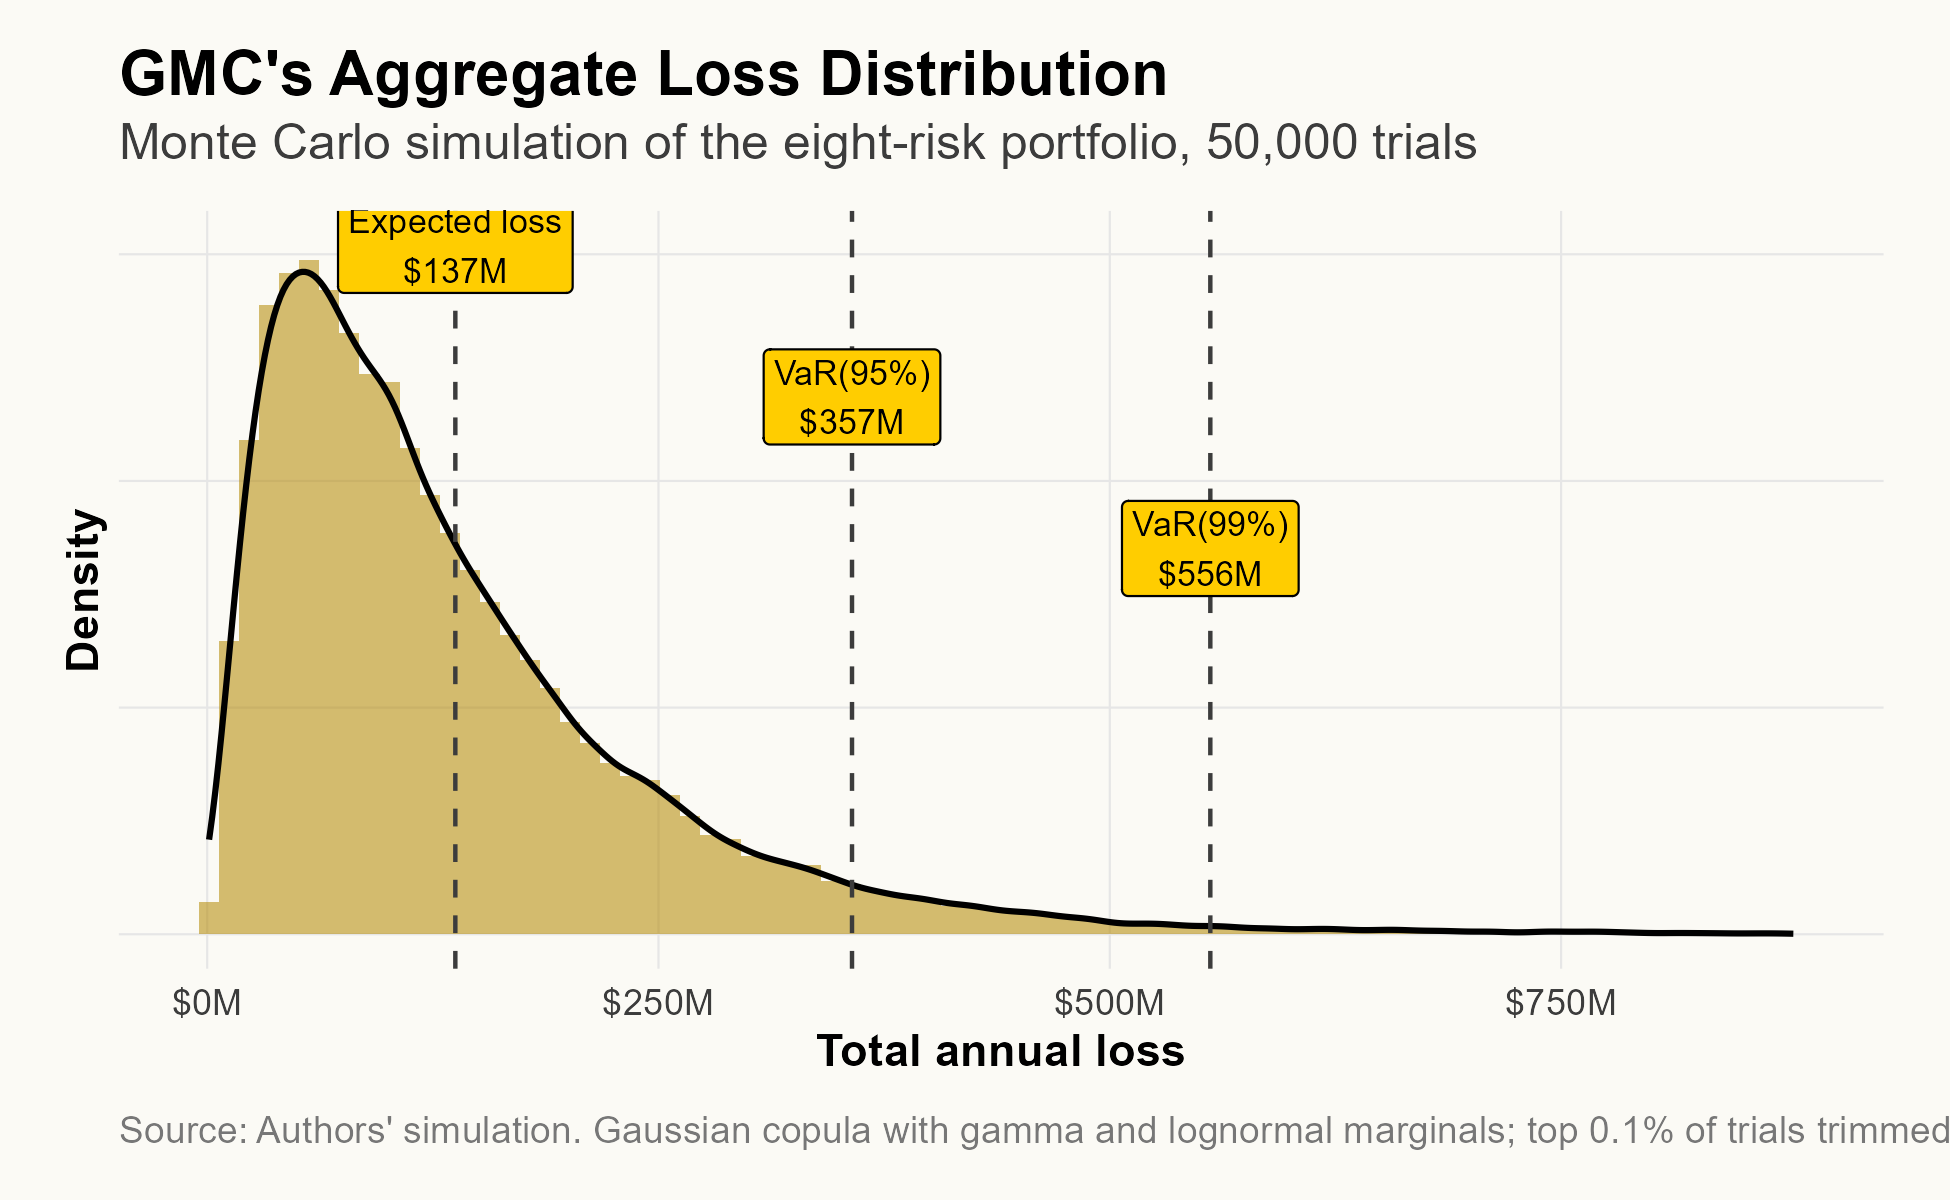
\includegraphics[width=\textwidth]{c6_aggregate_loss.png}
\column{0.34\textwidth}
\begin{itemize}
  \item Monte Carlo, 50{,}000 trials: Gaussian copula, gamma and lognormal marginals
  \item Strongly right-skewed: mean \$137M, VaR(95\%) = \$357M
  \item VaR(99\%) = \$556M --- over \$100M beyond the normal approximation
  \item The extreme tail is dominated by modeling choices, not data --- stress testing takes over there
\end{itemize}
\end{columns}
\end{frame}

\begin{frame}{GMC: Stress Results and Management Actions}
\begin{itemize}
  \item Severe recession: \$475M --- exceeds appetite, consumes a quarter of equity. Supply chain crisis: \$510M --- threatens covenants. All risks at 90th percentile: \$380M --- slightly over appetite.
  \item The agenda the analysis drives:
  \begin{itemize}
    \item Mitigate: higher property limits, supplier diversification, more commodity hedging
    \item Capital: hold equity; \emph{defer acquisitions} --- any new deal pushes VaR above appetite
    \item Monitor: quarterly portfolio VaR to the board; semi-annual stress tests; watch correlations
    \item Allocate: economic capital by marginal VaR; RAROC vs.\ a 12\% hurdle in segment incentives
  \end{itemize}
  \item The board sees its total risk position relative to appetite --- which is precisely what ERM is for.
\end{itemize}
\end{frame}

\section{Making It Work}

\begin{frame}{Implementation: The Hard Problems Are Organizational}
\begin{columns}[T]
\column{0.48\textwidth}
\textbf{Data and models}
\begin{itemize}
  \item Inconsistent metrics across silos --- standardize (e.g., all risks as VaR(95\%, annual))
  \item Thin loss histories for cyber, strategic, reputational risks
  \item Model risk: validate independently, backtest, present ranges not false precision
\end{itemize}
\column{0.48\textwidth}
\textbf{Organization and culture}
\begin{itemize}
  \item Silos resist the enterprise view --- a central ERM function with real authority, CRO dotted-line to the board
  \item ``My risk is unique'' syndrome --- common framework, with risk owners engaged in estimation
  \item Capital discipline meets politics --- transparency first, then link to capital and pay
\end{itemize}
\end{columns}
\medskip
What changed at Maersk after NotPetya was not just technology but \emph{authority}. Better --- and far cheaper --- to make that shift before the shock.
\end{frame}

\begin{frame}{Discussion Questions}
\begin{enumerate}
  \item Distinguish correlation from tail dependence. Why does tail dependence matter even when normal-period correlations are low --- and how does Maersk illustrate the distinction?
  \item Two risks each have expected loss \$20M and SD \$10M. Compute portfolio expected loss and SD for $\rho = 1.0$, $0.5$, and $0$. Interpret the diversification benefit in each case.
  \item Two acquisitions each have standalone VaR(95\%) = \$50M; one correlates 0.8 with your portfolio, the other 0.2. Without calculating, which adds more portfolio risk, and why?
  \item A board member says: ``With limited risk capacity, we should reduce every risk as much as possible.'' Using portfolio concepts, explain what's wrong with this --- and what the board should focus on instead.
\end{enumerate}
\end{frame}

\end{document}
